%  LP: la partie commentee ci-dessous a ete copié dans le fichierA
%  ``reference_flux.tex'' (peut etre supprimee ici)

%\subsubsection{Reference flux densities of secondary calibrators}
%\label{se:fluxSec}
%(revised by JFL Aug 2017 - must remove the old version in photometry-HA.tex)
%

%++ SPIRE refer.


%% Shortened version by LP, the original version can be found in the appendices


\section{Consistency test using aperture photometry {\color{blue} Jean-Fran\c cois}}
\label{se:aperture_photometry}

As a consistency check of the baseline calibration results that rely on PSF fitting, we have also used aperture photometry to recover as much as possible of the calibrator flux spread over the main beam and side
lobes of the telescope when assessing the stability of the calibration. 
For this study, observations were beammaps and $8' \times 5'$ otf's of the primary calibrators Uranus and Neptune
and of the secondary calibrators MWC349A, NGC7027 and CRL2688. All are
point-sources or quasi, except NGC7027 which is slightly extended.

% LP summary
We have implemented an aperture photometry relying on the estimation
of the total solid angle of the beam. The detailed description of the
aperture photometry method is given in
Sect.~\ref{ap:aperture_photometry_method}, and the determination of
the total beam solid angle is discussed in
Sect.~\ref{ap:aperture_photometry_solang}.

First, we have checked the stability of the primary calibrator fluxes
using aperture photometry, as described in
Sect.~\ref{ap:aperture_photometry_primary}. Here, we summarise the
results of the secondary calibrator flux stability cross-checks using
aperture photometry. An extended discussion of this study can be found
in Sect.~\ref{ap:aperture_photometry_secondary}.



We use MWC349A, NGC7027 and CRL2688 observations during runs N2R9 and N2R10.
Thirteen  of the 84 observations (sequence of 4 consecutive 4 min long
otf's) of these three secondary calibrators were discarded because
aperture photometry failed.

Secondary calibrator scans were reduced using the calibration
implemented in {\it kidpar-best3files-FXDC0C1-GaussPhot} for run 9 and
{\it kidpar-n2r10-calib} for run 10.
Maps of the secondary calibrators were produced and their
flux densities  were measured with two methods : aperture photometry
in Table~\ref{tab:flux_sec_Ap},
and  the pipeline Gaussian fit in Table~\ref{tab:flux_sec_NK}.
For aperture photometry, the solid angle of the total beam $\Omega_{true}$
was determined for each observation, while for the pipeline Gaussian
photometry a fixed solid angle is assumed
and based on the reference FWHM $12.5''$ and $18.5''$.
\footnote {Although flux densities  $S_{\nu}$ were measured at 
the central frequencies of the arrays $\nu_c$ (255, 152, 258 GHz) adopted initially for
the kidpars of Table~\ref{tab:Pipe}, they were changed afterward to the NIKA2 reference
frequencies  $\nu_{ref}$  (150, 260GHz) in using  the correction 
$\Delta S_{\nu}  = \alpha S_{\nu} (\nu_{ref}-\nu_c)/\nu_c $) with the spectral indices $\alpha$ 
($S_{\nu} \propto \nu^{\alpha}$) of the calibrators in Table~\ref{tab:flux_ref_sec}. These changes are less than 5\%.}
Color-corrections have been applied
with indices $\alpha=+0.6$, $-0.34$ and $+2.44$ for MWC349A, NGC7027 and CRL2688, respectively, while Uranus and
Neptune have $\alpha=+1.6$. These color corrections are smaller than 2.5\% (see Table in
\S~\ref{se:cal_HA}, CAUTION : this table is pending in  HA section).  
%Again, both of these corrections are included in Tables~\ref{tab:flux_sec_Ap} and \ref{tab:flux_sec_NK} 
%where the flux densities and uncertainties are the mean and rms of all observations of each source during each run. 
Note that in Tables~\ref{tab:flux_sec_Ap} and \ref{tab:flux_sec_NK}, for each calibrator, its
flux density and uncertainty  are  the mean and
standard deviation of all its observations with an array during a run.   
Note again that each observation is the integration of 4 consecutive otf scans (total 16 minutes). 

\begin{table}[th]
\begin{center}
\begin{tabular}{|c|c|c|c|c|c|}
\hline
\multicolumn{3}{|c}{}  & \multicolumn{3}{|c|}{Flux densities (Jy)}   \\
\hline
         & run  & \#obs &  A1                    &  A2                   &    A3                    \\
         &      &      &  $S_{260 {\rm GHz}}$     &  $S_{150 {\rm GHz}}$  & $S_{260 {\rm GHz}}$    \\
\hline\hline
MWC349A   &  9   & 10  &  $2.23\pm0.32$  ($+8.2\%$)  &  $1.49\pm0.11$ ($+0.6\%$) &  $2.15\pm0.35$ ($+4.6\%$)      \\
  $''$   & 10   & 14  &  $1.96\pm0.17$  ($-4.8\%$)  &  $1.48\pm0.08$ ($+0.2\%$) &  $2.10\pm0.19$ ($+1.8\%$)                  \\ 
  \hline
NGC7027  &  9   & 13  &  $3.22\pm0.39$  ($-6.9\%$)  &  $4.19\pm0.18$ ($-1.6\%$) & $3.05\pm0.54$  ($-11.9\%$)      \\
  $''$   & 10   & 15  &  $3.01\pm0.36$  ($-13.0\%$) &  $4.04\pm0.30$ ($-5.2\%$) & $3.31\pm0.19$  ($-4.2\%$)                   \\ 
  \hline
CRL2688  &  9   & 11  &  $2.91\pm0.48$  ($-0.1\%$)  &  $0.59\pm0.05$ ($-22.9\%$)  &  $2.68\pm0.51$ ($-7.9\%$)     \\
  $''$   & 10   &  8  &  $2.36\pm0.14$  ($-19.0\%$) &  $0.52\pm0.04$ ($-32.1\%$)  &  $2.49\pm0.18$ ($-14.5\%$)                   \\
\hline
\end{tabular}
\caption[Flux densities from aperture photometry]{Flux densities from aperture photometry and relative differences with respect to reference values.}
\label{tab:flux_sec_Ap}
\end{center}
\end{table}
%open(1,file='sequence_Ur_Nep_r_8_9_10.dat' (contient aussi cal sec du r 9 seulement)  ;  flux=flux
% open(1,file='run10_cal_sec.dat')    ! kidpar_n2r10_calib (mask=50") with F2D, bramax (seul fichier avec cela)    
% cahier II p. 46, 47 : corrections (255, 258GHz) --> 260GHz  (152GHz) --> 150GHz  and color-correction with Table p.37


% LP: obsolete because relying on an old version of the pipeline photometry

%\begin{table}[bh]
%\begin{center}
%\begin{tabular}{|c|c|c|c|c|c|}
%\hline
%\multicolumn{3}{|c}{}  & \multicolumn{3}{|c|}{Flux  densities (Jy)}   \\
%\hline\hline
%         & run  & \#obs &  A1                        &  A2                        &           A3                  \\
%         &      &       &  $S_{260 {\rm GHz}}$       &  $S_{150 {\rm GHz}}$       & $S_{260 {\rm GHz}}$         \\
%\hline  
%MWC349   &  9   & 10    &  $1.98\pm0.16$ ($-4.1\%$)  &  $1.46\pm0.05$ ($-1.3\%$)  &  $2.02\pm0.17$ ($-2.0\%$)     \\
%  $''$   & 10   & 14    &  $1.71\pm0.16$ ($-16.8\%$) & $1.44\pm0.05$ ($-2.5\%$)   &  $1.84\pm0.20$ ($-10.7\%$)      \\ 
%  \hline
%NGC7027  &  9   & 13    &  $3.53\pm0.33$ ($+2.1\%$)  &  $4.28\pm0.18$ ($+0.4\%$)  & $3.62\pm0.36$ ($+4.7\%$)      \\
%  $''$   & 10   & 15    &  $3.27\pm0.19$ ($-5.5\%$)  & $4.28\pm0.14$ ($+0.6\%$)   &  $3.53\pm0.19$ ($+2.1\%$)        \\ 
%  \hline
%CRL2688  &  9   & 11    &  $2.53\pm0.23$ ($-17.0\%$) &  $0.55\pm0.02$ ($-27.5\%$) &  $2.49\pm0.24$ ($-14.2\%$)    \\
%  $''$   & 10   &  8    &  $2.22\pm0.12$ ($-23.6\%$) &  $0.54\pm0.02$ ($-29.3\%$) &  $2.32\pm0.13$ ($-20.4\%$)     \\
%\hline
%\end{tabular}
%\caption[Flux densities from pipeline gaussian fit]{ and relative differences  with respect to reference values.}
%\label{tab:flux_sec_NK}
%\end{center}
%\end{table}
%open(1,file='sequence_Ur_Nep_r_8_9_10.dat' (contient aussi cal sec du run 9 seulement) ;   flux=S_NK
% open(1,file='run10_cal_sec.dat')    ! kidpar_n2r10_calib (mask=50") with F2D, bramax (seul fichier avec cela) 

\noindent {\bf FM: i'm not sure that the relative differences with respect to reference values is an interesting parameters as in our case 
the bias, if any, is small than the error bars.}\\

\noindent {\bf FM: I think it would help the reader to have the values of these tables on a figure (or 2) to judge by eye is there is an
agreement. Moreover, the comparison requires to use a table given 10 pages before. The assessment of the photometry is a key point that would deserve an illustration. (but keep the tables as well}\\

\noindent {\bf JFL reply to FM : OK, in a short while, I will make a plot to summarize  the two tables and will remove \% differences
  from Tables (but they are kept in in the meantimes}\\

By inspection of Table~\ref{tab:flux_sec_Ap}, we conclude that :

\begin{itemize}
  
\item measured flux densities are statistically consistent when results are compared between runs 9 and 10 despite very different weather conditions.
Satisfactorily, this is an indication that the atmospheric signal is properly removed from the raw data by the pipeline.   


\item   measured flux densities are biased at the  10\% level when results are compared between the two methods
(aperture photometry and pipeline Gaussian photometry) ;
for each calibrator,  it is 10\% up for MWC349A and CRL2688 (point sources) while it is 10\% down
for NGC7027 (slightly extended) and it is similar for the three arrays.
This bias between the two methods should be investigated further but it indicates
already that the two methods are viable. We remind that the
pipeline fits the source with a Gaussian with a reference FWHM empirically fixed to $12.5''$ or $18.5''$, {\it i.e.} larger than the main beam width
in order to approximate the complexe profile of the beam.  

\item measured flux densities of MWC349A and NGC7027 are statistically consistent when compared to the reference flux densities of
Table~\ref{tab:flux_ref_sec}. This is not true
     for CRL2688 which is found to be 20\% lower at 1mm and 30\% lower at 2mm. This overestimation of the reference flux densities
      in Table~\ref{tab:flux_ref_sec} is likely due to the large lever arm in frequency when extrapolating from
      the SCUBA2 850 $\mu$m (345 GHz) and 450 $\mu$m (650 GHz) measurements to the NIKA2 frequencies 150 and 260~GHz,
      and because of the large uncertainty of  the SCUBA2 450 $\mu$m flux density.
      However, we note again that the NIKA2 flux densities of CRL2688 are satistically consistent between the two runs.
      Future measurements should be planned
      for confirmation of this stability before CRL2688 is considered a reliable calibrator.

\end{itemize}

Finally, we provide the ratios between measured and reference flux densities for MWC349 only because
its reference flux densities are monitored at PdB
by IRAM at frequencies close to NIKA2 and so are the most reliable among the three secondary calibrators.
Ratios are given for aperture photometry in Fig.~\ref{fig:ratio_349_Ap}, and  given for
the pipeline Gaussian photometry in Fig.~\ref{fig:ratio_349_NK}.
The mean ratio and rms are provided in the figures. At 1mm, rms are $\sim$~10\% on arrays A1 and A3 
and are slightly better in using the pipeline Gaussian photometry than aperture photometry.
%However, for the  pipeline Gaussian photometry, the mean ratios are
%systematically lower than unity by $\sim$~10\% at 1mm.
%This bias in using the pipeline Gaussian photometry
%is also found for the Uranus and Neptune data of runs 9 and 10 but at
%a level of 5\% at both bands. It is likely that an adjustement
%of the reference FWHMs for the pipeline Gaussian fit (currently $12.5''$ and $18.5''$) could remove this bias.


%\subsection{Tentative gain-elevation curve}

%We have searched for any elevation dependence of the solid angle of the total beam  $\Omega_{true}$ of Uranus and Neptune
%and found none for
%the elevation range of their observations between  30$^{\circ}$ and 65$^{\circ}$.  We have also studied such a dependence
%for the observations of the three secondary calibrators which span a larger range between elevations 23$^{\circ}$ and 74$^{\circ}$.
%The most conclusive study is for NGC7027, the brightest secondary calibrator, in Figure~\ref{fig:gain_curve_NG7027}. 
%Its pipeline Gaussian photometry exhibits some degree of curvature centered around elevation 45$^{\circ}$ and in a similar way
%for the three arrays.
%While the pipeline Gaussian photometry  assumes a fixed solid angle for the total beam based on the reference FWHM's $12.5''$ and $18.5''$,
%the solid angle as determined with the data themselves in using
%eq.~\ref{eq:Otrue} exhibits instead a similar curvature centered on elevation 45$^{\circ}$. This needs confirmation with further
%observations  over the largest elevation range possible at the telescope and on the strongest source available. Note finally,
%that the flux density of NGC7027 determined
%with aperture photometry does not exhibit any curvature, as expected, since the conversion factor ${dx^2} \over {\Omega_{true}}$
%in eq~\ref{eq:ApPh} models the effect.  We stress again that the EMIR gain curved was not turned on to process the data. 





%From these two tables, we conclude that  the 2 mm flux densities of MWC349A and NGC7027 measured with array 2 are consistent with predictions,
%and consistent between runs (9 and 10) and methods (aperture photometry, pipeline Gaussian fit) at the few percent level
%($(S_{meas}-S_{ref})/S_{ref} \times 100)$. But this is not the case for CRL2688.  Its NIKA2 2mm
%flux density is $\sim$25\% lower than prediction, consistently between runs and methods. Hence, this may be due to an over estimation
%in the prediction of the 2 mm flux density that was extrapolated from the SCUBA2 850 $\mu$m and 450 $\mu$m measurements
%and because of the large lever arm in frequency. We note this
%over estimation seems to be also true at 1mm for this source in the two Tables.
%Future observations of CRL2688 will check wether or not its new NIKA2 flux densities are valid to populate usefully its SED
%for science purpose. {\bf FM : so the conclusion is that it is not a reliable calibrator and we should not use it hereafter}

%For the 1 mm flux densities of MWC349 and NGC7027 from these two tables, we conclude that their  measurements with arrays 1 and 3 are
%at the 10\% level   ($(S_{meas}-S_{ref})/S_{ref} \times 100)$  and are consistent with statistical uncertainties estimated from
%the rms of their fluctuations
%during the two runs and shown in Fig.~\ref{fig:ratio_cal_sec}. 


%{\bf FM: {\it at the 10\% level} was said to be {\it the few percent level} a few lines above.}\\

%{\bf FM: i would suggest to remove CRL2688 from Fig.~\ref{fig:ratio_cal_sec}. From the discussion of the text we conclude that it can not be used for calibration as the
%    flux at 1 and 2 mm my be biased due to the extrapolation. This way we can conclude from the figure that NIKA2 photometry is at the 10\%
%    level.}\\
    
%    {\bf FM: i would suggest to change the scale in Fig.~\ref{fig:ratio_cal_sec} as we want to show a 10\% effect...}\\
    
%    {\bf FM: for Fig.~\ref{fig:ratio_cal_sec} histograms would be a better choice as we want to evaluate by eye, the rms, the agreement
%    with one of this ratio of values. Moreover, effect of  weather conditions (tau) is shown on fig. \ref{fig:corr_cal_sec}}\\

%For example, NGC7027, A1, run 10, aperture photometry in Table~\ref{tab:flux_sec_Ap}
%yields  :

%$$rms(S_{obs})/<S_{obs}>=0.36Jy/3.01Jy \times 100=11.9\%$$

%\noindent which is statistically consistent with :

%$$|(S_{meas}-S_{ref})/S_{ref}| \times 100=15.0\%~,$$

%\noindent where $S_{meas} = <S_{obs}>$.

%Finally, we have plotted the flux density ratios versus elevation, opacity and attenuation  for three
%secondary calibrators in  Fig.~\ref{fig:corr_cal_sec}. No clear correlation is apparent.


%{\bf FM: you should say whether pipeline or aperture value is used for the ratio}\\


%{\bf FM: by the way, a conclusion on pipeline versus aperture values would be useful regarding future use of the pipeline. (no need to
%perform aperture evaluation ?)}\\


\begin{figure}[p]
\begin{center}
  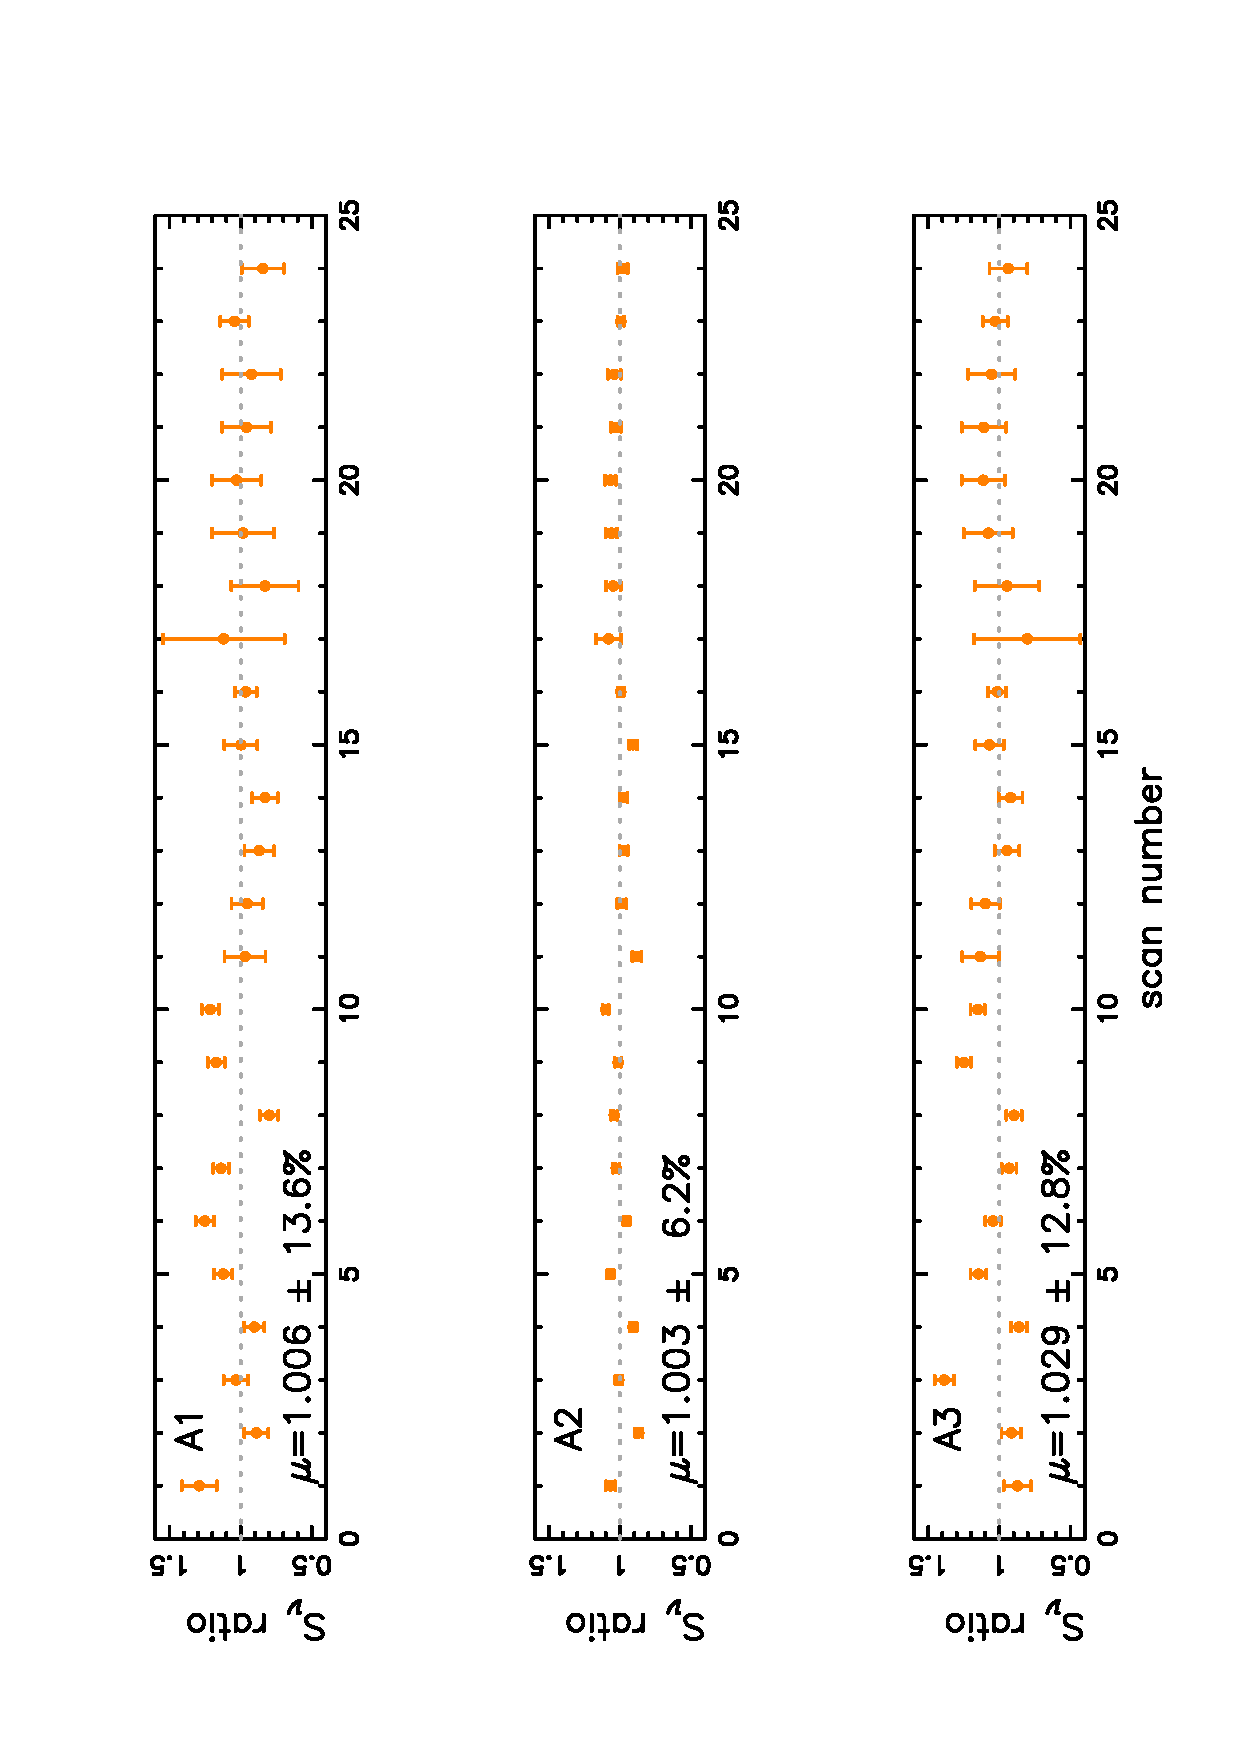
\includegraphics[clip, angle=-90, scale=0.6]{Figures/Ratio_vs_index_MWC349_r9_r10_Ap.pdf}
  \caption[Aperture photometry flux density stability checks on secondary calibrators]{Ratios between measured and reference flux densities of  the secondary calibrator  MWC349A
    during runs 9 and 10.  The flux density is measured with aperture photometry. Note that mean ratios
    on the three arrays are close to unity as expected for proper calibration.
    Scan numbers are time ordered (index 1 to 11 : run 9 (fair weather) and index 12 to 24 : run 10 (mediocre weather).
    Each observation is a sequence of 4 consecutive 4 minute long otfs (total integration is 16 minutes).
  }
\label{fig:ratio_349_Ap}
\end{center}
\end{figure}



% LP: old version of the pipeline photometry = obsolete
%\begin{figure}[p]
%\begin{center}
%  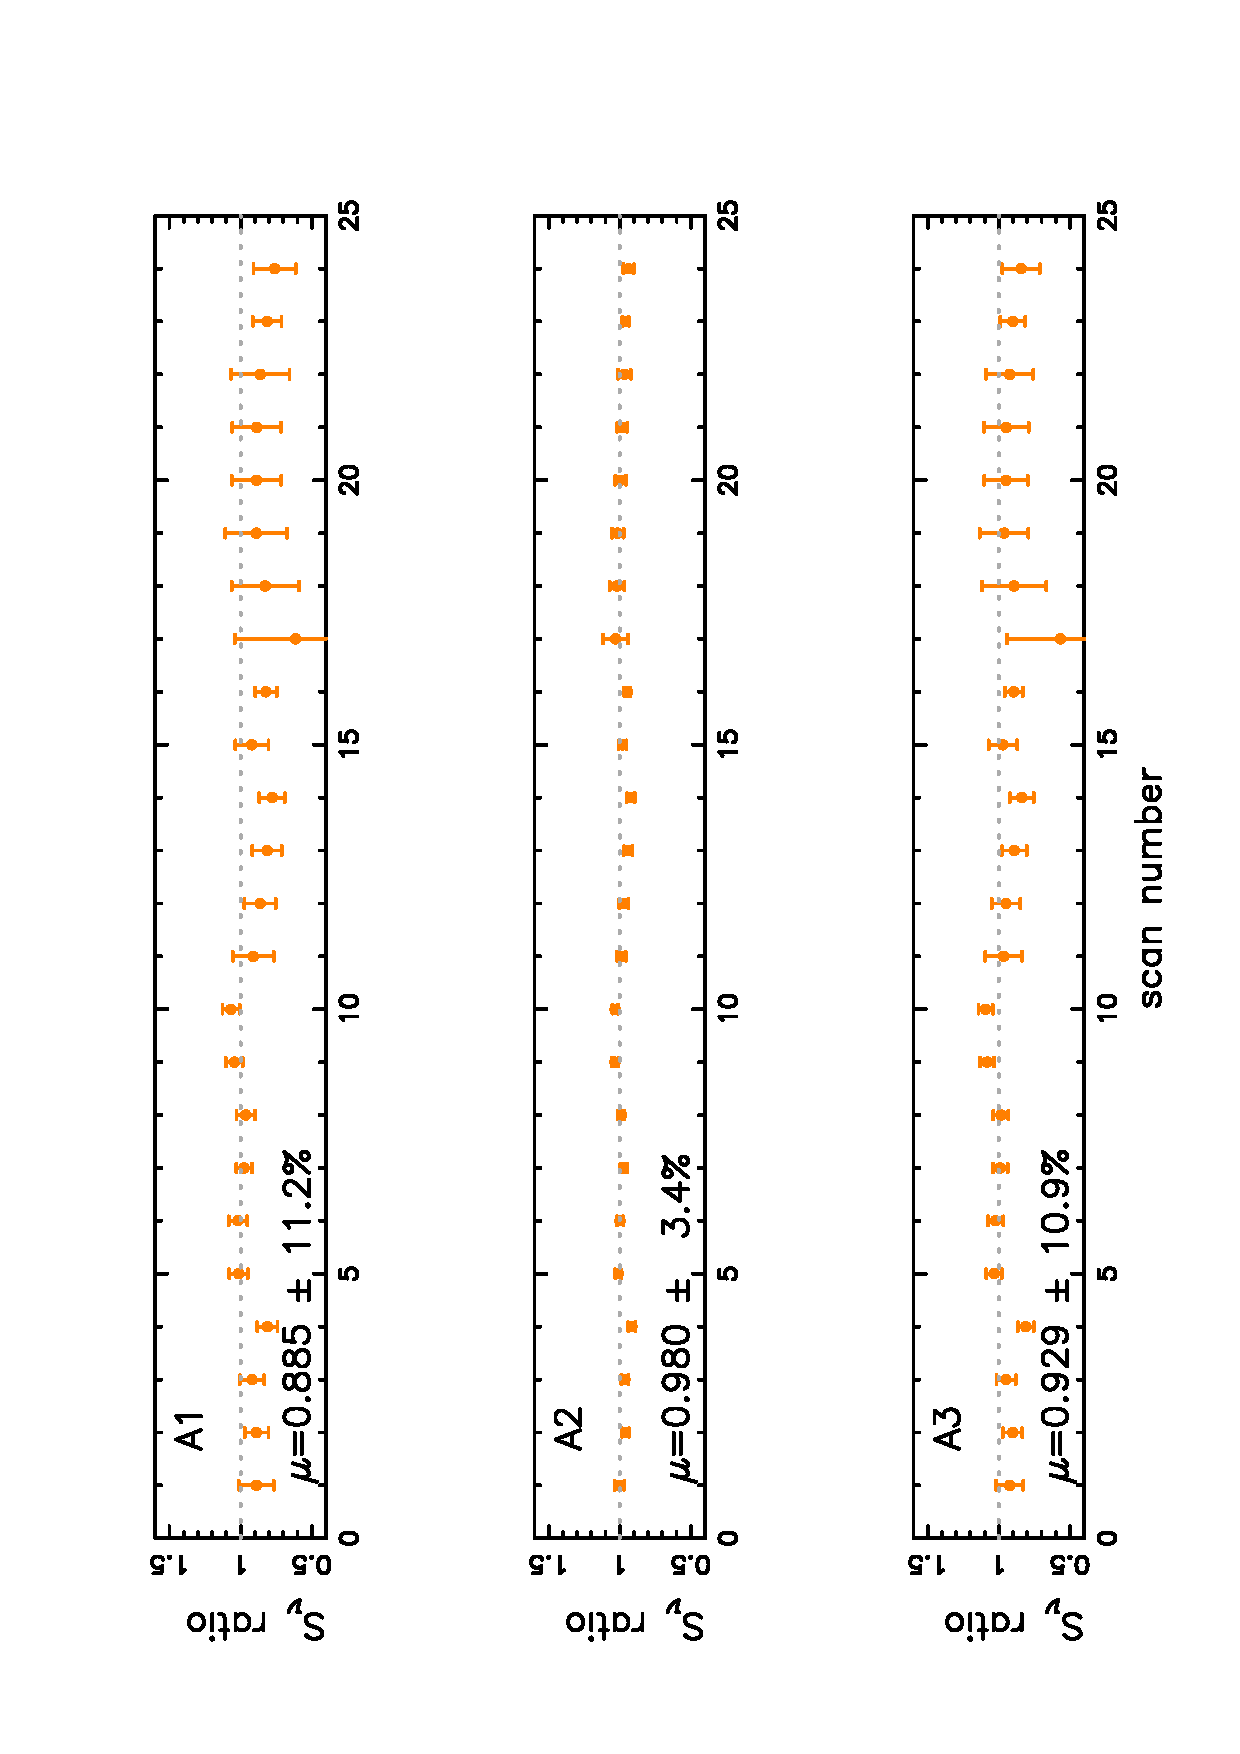
\includegraphics[clip, angle=-90, scale=0.6]{Figures/Ratio_vs_index_MWC349_r9_r10_NK.pdf}
%  \caption[Fixed-Gaussian flux density stability checks on secondary calibrators] {Ratios between measured and reference flux densities of  the secondary calibrator  MWC349A 
%    during runs 9 and 10.  {\bf The flux density is measured with the Pipeline Gaussian photometry}. Note that mean ratios 
%    on A1 and A3 are $\sim$~10 \% lower than unity, unsatisfactorily.
%    Scan numbers are time ordered (index 1 to 11 : run 9 (fair weather), and index 12 to 24 : run 10 (mediocre weather).
%    Each observation is a sequence of 4 consecutive 4 minute long otfs (total integration is 16 minutes).
%  }
%\label{fig:ratio_349_NK}
%\end{center}
%\end{figure}





















